\begin{abstract}												
\begin{minipage}{0.48\textwidth} \begin{flushleft}

\includegraphics[scale = 0.09]{images/ipn}
\end{flushleft}\end{minipage}
\begin{minipage}{0.48\textwidth} \begin{flushright}
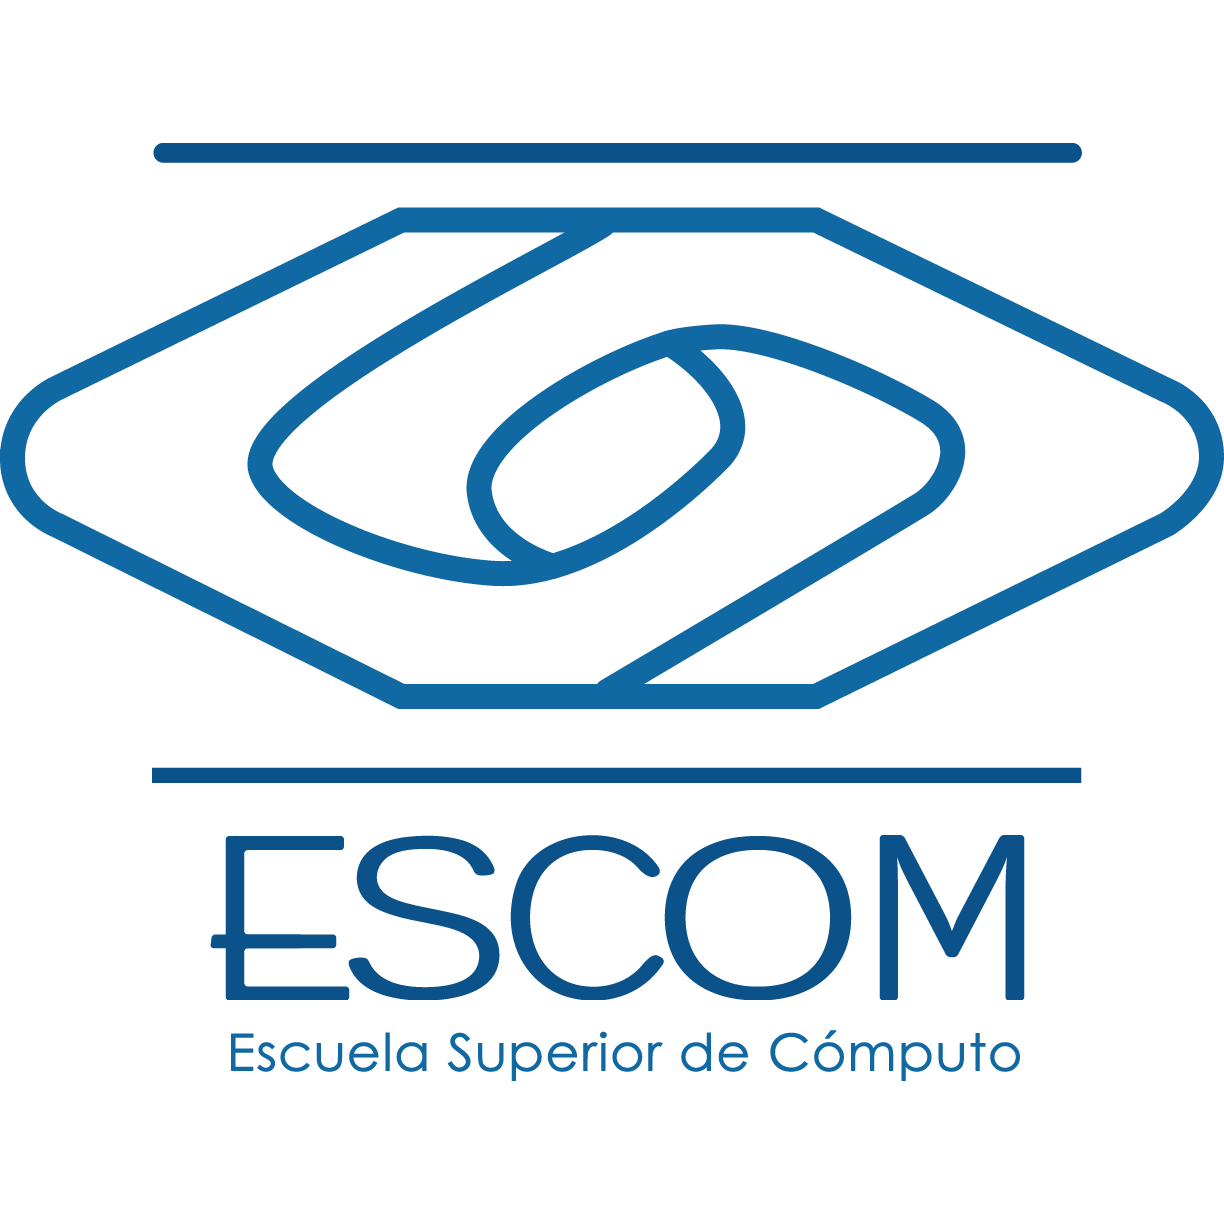
\includegraphics[scale = 0.08]{images/escom}
\end{flushright}\end{minipage}

El presente proyecto consiste en desarrollar un software que está enfocado a la enseñanza, aprendizaje y demostración del cuerpo humano mediante Realidad Virtual (R.V.), el mismo que puede ser usado en la Escuela Superior de Medicina (E.S.M.) y Escuela Nacional de Medicina y Homeopatía (E.N.M. y H.) en las áreas de Morfología y Anatomía como soporte para la enseñanza de las áreas antes mencionadas. 
\\
De esta manera se espera aumentar el número de herramientas que poseen los estudiantes de medicina y reforzar el aprendizaje del alumnado con tecnología actual, escalable, con mayor disponibilidad y facilidad de uso, en contraste con el uso de cadáveres humanos.
\\[4cm]
\textbf{Palabras clave} - Animación por Computadora, Gráficos por Computadora, Realidad Virtual, Estudio Multimedia
\\[2cm]
\textbf{Presenta:}
\\[0.5cm]
Almendarez Perdomo Rodrigo
\\[2cm]
\textbf{Directores}
\\[0.5cm]
M. en Ing. Moscoso Malagón Yosafat
\\
M. en C. Saucedo Delgado Rafael Norman
\\
\end{abstract}							
